\documentclass[a4paper,10pt]{article}
\usepackage[utf8]{inputenc}
\usepackage[english]{babel}
\usepackage{float}
\usepackage{graphicx}
\usepackage{caption}
\usepackage{subcaption}
\usepackage{amsmath}
\usepackage{multirow}
\usepackage{algorithm}
\usepackage{algorithmic}
% \usepackage{algorithmicx}

%opening
\title{Protein Classes Library}
\author{}

\begin{document}

\maketitle

\section{Introduction}
Protein folding is a problem of predicting the atomic structure of a protein given its amino-acid sequence. 
The challenging part of this problem is the complexity of the manifold to which belongs a protein structure.
The key idea of the library is the local conversion of this manifold to the euclidian space, where deep learning
techniques can be applied. After some machine learning algorithm provides prediction of the folding step in this 
local space, we have to convert this step back to the changes of the coordinates on the manifold.

\section{AB Protein Model}

\subsection{From Manifold to Euclidian space}

Figure \ref{Fig:proteinModelCalpha} represents the model we use to describe a protein conformation. In this 
model only C-$\alpha$ atoms are used. The distance between them assumed to be constant ($R_{C\alpha - C\alpha}=1.0\AA$).

\begin{figure}[H]
    \centering
    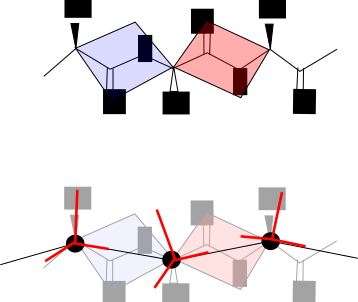
\includegraphics[width=\linewidth]{Fig/amide_planes.png}
    \caption{The model of protein using C-$\alpha$ atoms in internal coordinates.}
    \label{Fig:proteinModelCalpha}
\end{figure}

The position of the next atom in the chain is obtained by:
\begin{itemize}
\item Translation along axis x by 1\AA 
$$
T_x = \begin{bmatrix}
1 & 0 & 0 & 1 \\
0 & 1 & 0 & 0 \\
0 & 0 & 1 & 0 \\
0 & 0 & 0 & 1
\end{bmatrix} 
$$
\item Rotation by the angle $\alpha$ around the x axis (dihedral angle)
$$
R_x = \begin{bmatrix}
1 & 0 & 0 & 0 \\
0 & cos(\beta) & -sin(\beta) & 0 \\
0 & sin(\beta) & cos(\beta) & 0 \\
0 & 0 & 0 & 1
\end{bmatrix} 
$$
\item Rotation by the angle $\beta$ around the z axis (bending angle)
$$
R_z = \begin{bmatrix}
cos(\alpha) & -sin(\alpha) & 0 & 0 \\
sin(\alpha) & cos(\alpha) & 0 & 0 \\
0 & 0 & 1 & 0 \\
0 & 0 & 0 & 1
\end{bmatrix} 
$$

\end{itemize}

The first atom is fixed at the origin of coordinates. The total transformation matrix will look like:
$$
R = R_z \cdot R_x \cdot T_x = 
\begin{bmatrix}
cos(\alpha) & -sin(\alpha)cos(\beta) & sin(\alpha)sin(\beta) & cos(\alpha)\\
sin(\alpha) & cos(\alpha)cos(\beta) & -cos(\alpha)sin(\beta) & sin(\alpha)\\
0 & sin(\beta) & cos(\beta) & 0\\
0 & 0 & 0 & 1
\end{bmatrix} 
$$


Suppose we have $N_{angles}$ angles in the protein, they correspond to $N_{angles}+2$ vectors. The position of the first 
vector is fixed and the last vector is parametrized by the previous angle. To compute their positions we
sequentially multiply them by $R(\alpha_i, \beta_i) = R^i$:
$$ r_{i+1} = R^0 \cdot R^1 \dots A^{i-1} \cdot R^{i} \cdot \begin{bmatrix} 0 \\ 0 \\ 0 \\ 1 \end{bmatrix}$$
During the forward pass we save the matrixes:
$$A_i = R^{0} \cdot R^{1} \dots R^{i-1} \cdot R^{i}$$
because they are useful during backward computation. The coordinates of the atoms can be computed:
$$r_{i+1} = A_i \cdot \begin{bmatrix} 0 \\ 0 \\ 0 \\ 1 \end{bmatrix}$$

Now, we need to compute gradients of the internal angles with respect to the cartesian coordinates.
Each $R^{i}$ matrix depends on the angles $\alpha_i$ and $\beta_i$ (lets denote them as $q_i$), 
therefore the derivative of the coordinates:
$$ \frac{dr_i}{dq_j} = \frac{d R^{0} \cdot R^{1} \dots R^{i-1} \cdot R^{i} \cdot r_0} {dq_j} = 
R^{0} \cdot R^{1} \dots \frac{dR^j}{dq_j} \dots R^{i-1} \cdot R^{i} \cdot r_0 $$
using $A$ matrixes we obtain:
$$ \frac{dr_i}{dq_j} = A_{j-1}  \cdot \frac{dR^j}{dq_j} R^{j+1} \dots R^{i} \cdot r_0 $$




\subsection{From Euclidian space to Manifold}
I will derive the derivatives of angles using simple analogy to the rigid body kinematics.
When we compute the derivative of a single angle with respect to the coordinates of a single atom, 
we assume all other angles constant, which means that the protein behaves as a rigid body on a joint.

\subsection{Bending angle}
Lets look at the Fig. \ref{Fig:BendingKinematics}. The change of atomic coordinate $\mathbf{r}_j = \mathbf{\widetilde{r}_j} + \mathbf{r_i}$ 
can be expressed using the angular velocity:
$$
\frac{d\mathbf{r}_j}{dt} = [\mathbf{\omega}, \mathbf{\widetilde{r}}_j]
$$

\begin{figure}[H]
    \centering
    \includegraphics[width=\linewidth]{Fig/BendingKinematics.png}
    \caption{The model of bending angle change upon changing an an atom coordinate.}
    \label{Fig:BendingKinematics}
\end{figure}

The angular velocity around the axis in the joint $i$ is the vector perpendicular to this joint and proportional to the change of the angle:
$$
\mathbf{\omega} = [\mathbf{u}, \mathbf{v}] \frac{d\alpha_i}{dt}
$$
where the vectors $\mathbf{u} = \mathbf{r}_i - \mathbf{r}_{i-1}$ and $\mathbf{v} = \mathbf{r}_{i+1} - \mathbf{r}_{i}$ should 
not be parallel (otherwise we chose an arbitrary vector and $\mathbf{u}$). We denote $\mathbf{w} = [\mathbf{u}, \mathbf{v}]$ 
and the changes in angle and coordinates can be written:
$$
\frac{d\mathbf{r}_j}{dt} = [\mathbf{w}, \mathbf{\widetilde{r}}_j] \frac{d\alpha_i}{dt}
$$
Now, lets use the following relation for tripple cross products: 
$[\mathbf{a},[\mathbf{b},\mathbf{c}]] = \mathbf{b} (\mathbf{a}, \mathbf{c}) - \mathbf{c} (\mathbf{a}, \mathbf{b})$
and
$(\mathbf{a},[\mathbf{b},\mathbf{c}]) = (\mathbf{c} [\mathbf{a}, \mathbf{b}]) = (\mathbf{b}, [\mathbf{c}, \mathbf{a}])$.
First we multiply both parts by the cross product:
$$
([\mathbf{w}, \mathbf{\widetilde{r}}_j], \frac{d\mathbf{r}_j}{dt}) = ([\mathbf{w}, \mathbf{\widetilde{r}}_j],
[\mathbf{w}, \mathbf{\widetilde{r}}_j]) \frac{d\alpha_i}{dt}
$$
and the we simplify the right part of the equation:
$$
([\mathbf{w}, \mathbf{\widetilde{r}}_j], [\mathbf{w}, \mathbf{\widetilde{r}}_j]) = (\mathbf{r}_j, [[\mathbf{w}, \mathbf{\widetilde{r}}_j], \mathbf{w}]) =
(\mathbf{\widetilde{r}}_j, \mathbf{\widetilde{r}}_j(\mathbf{w},\mathbf{w}) - \mathbf{w}(\mathbf{w},\mathbf{\widetilde{r}}_j))
$$
Taking into account that we normalized the vector $\mathbf{w}$ we write:
$$
([\mathbf{w}, \mathbf{\widetilde{r}}_j], \frac{d\mathbf{r}_j}{dt}) = \left( |\mathbf{\widetilde{r}}_j|^2 - 
(\mathbf{\widetilde{r}}_j,\mathbf{w})^2 \right) \frac{d\alpha_i}{dt}
$$
The expression on the right is the square of torque. Now we can take individual components of the derivatives and divide them:
$$
\frac{d\alpha_i^k}{dr^k_j} = \frac{[\mathbf{w}, \mathbf{\widetilde{r}}_j]_k}{|\mathbf{\widetilde{r}}_j|^2 - (\mathbf{\widetilde{r}}_j,\mathbf{w})^2}
$$
Now special care should be payed to the case when $\mathbf{\widetilde{r}}_j = \mathbf{0}$. 
In this case we take $\mathbf{\widetilde{r}} = \mathbf{v}$ for the right body and 
$\mathbf{\widetilde{r}} = \mathbf{u}$ for the left one. Also, 
the direction of the vector $\mathbf{w}$ depends on the body, where point $j$ is located. 
Altogether these two body motions can be expressed like this:
$$
\frac{d\alpha_i^k}{dr^k_j} = \frac{ -h_{ij}[\mathbf{w},\mathbf{\widetilde{r}}]_k}{|\mathbf{\widetilde{r}}|^2 - (\mathbf{\widetilde{r}},\mathbf{w})^2} + 
\frac{ h_{ji}[\mathbf{w},\mathbf{\widetilde{r}}]_k}{|\mathbf{\widetilde{r}}|^2 - (\mathbf{\widetilde{r}},\mathbf{w})^2}
$$ where
$$
h_{ab} = \left \{ \begin{array}{lll}
+1  & a\geq b \\
0  & a<b
\end{array}
\right.
$$

Or algorithmically:
\begin{algorithm}
    \caption{Bending matrix computation}
    \label{alg:BendingAlgorithm}
    \begin{algorithmic}
        \FOR {$i = 0 \dots N$ scanning bending angles} 
            \FOR {$j = 0 \dots N+2$ scanning atoms} 
                \IF {$j < i+1 $ (atom $i+1$ corresponds to the angle $i$, left body)}
                    \STATE $\mathbf{\widetilde{r}} = \mathbf{r}_j - \mathbf{r}_{i+1}$
                    \STATE $\mathbf{w} = [\mathbf{r}_{i+2} - \mathbf{r}_{i+1}, \mathbf{r}_{i} - \mathbf{r}_{i+1}]$
                    \STATE $\frac{d\alpha_i^k}{dr^k_j} = \frac{[\mathbf{w},\mathbf{\widetilde{r}}]_k}{|\mathbf{\widetilde{r}}|^2 - (\mathbf{\widetilde{r}},\mathbf{w})^2}$
                \ELSIF {$j > i+1 $ (atom in the right body)}
                    \STATE $\mathbf{\widetilde{r}} = \mathbf{r}_j - \mathbf{r}_{i+1}$
                    \STATE $\mathbf{w} = [\mathbf{r}_{i} - \mathbf{r}_{i+1}, \mathbf{r}_{i+2} - \mathbf{r}_{i+1}]$
                    \STATE $\frac{d\alpha_i^k}{dr^k_j} = \frac{[\mathbf{w},\mathbf{\widetilde{r}}]_k}{|\mathbf{\widetilde{r}}|^2 - (\mathbf{\widetilde{r}},\mathbf{w})^2}$
                \ELSIF {$j = i+1$ (atom is the joint center) }
                    \STATE Left body
                    \STATE $\mathbf{\widetilde{r}} = \mathbf{r}_{i+1} - \mathbf{r}_{i}$
                    \STATE $w = [\mathbf{r}_{i} - \mathbf{r}_{i+1}, \mathbf{r}_{i+2} - \mathbf{r}_{i+1}]$
                    \STATE $\frac{d\alpha_i^k}{dr^k_j} = \frac{[\mathbf{w},\mathbf{\widetilde{r}}]_k}{|\mathbf{\widetilde{r}}|^2 - (\mathbf{\widetilde{r}},\mathbf{w})^2}$
                    \STATE Right body
                    \STATE $\mathbf{\widetilde{r}} = \mathbf{r}_{i+1} - \mathbf{r}_{i+2}$
                    \STATE $w = [\mathbf{r}_{i+2} - \mathbf{r}_{i+1}, \mathbf{r}_{i} - \mathbf{r}_{i+1}]$
                    \STATE $\frac{d\alpha_i^k}{dr^k_j} += \frac{[\mathbf{w},\mathbf{\widetilde{r}}]_k}{|\mathbf{\widetilde{r}}|^2 - (\mathbf{\widetilde{r}},\mathbf{w})^2}$
                \ENDIF               
            \ENDFOR
        \ENDFOR
    \end{algorithmic}
\end{algorithm}

% \subsection{Dihedral angle}

\begin{figure}[H]
    \centering
    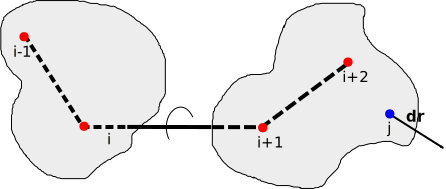
\includegraphics[width=\linewidth]{Fig/DihedralKinematics.png}
    \caption{The model of dihedral angle change upon changing an an atom coordinate.}
    \label{Fig:DihedralKinematics}
\end{figure}

Here, the derivation for the points in two bodies that do not lie on the line $i, i+1$ is essentially the same. Except
we already have a fixed rotation axis $\mathbf{w} = \frac{\mathbf{r}_{i+1} - \mathbf{r}_i}{|\mathbf{w}|}$, which is 
negative for the left body and positive for the right one.
The movement of point $i$ and $i+1$ requires special treatment deserves: in this case the rotation axis moves itself.
The angle of rotation can be computed as follows:
$$
\beta = \arccos \left( \frac{ \left([\mathbf{u}, \mathbf{w}], [\mathbf{w}, \mathbf{v}] \right) }{\sin(\alpha_{i-1}) \sin(\alpha_{i})} \right)
$$
In this case I took the expressions from MODELLER \cite{}:
$$
\begin{array}{lcl}
\frac{d\beta_i}{dr_{i}} &=& -\frac{1}{\sin(\beta)} \left( [\mathbf{r}_{i,i+1}, \mathbf{a}] - [\mathbf{r}_{i+1,i+2}, \mathbf{b}] \right) \\
\frac{d\beta_i}{dr_{i+1}} &=& -\frac{1}{\sin(\beta)} \left( [\mathbf{r}_{i,i+2}, \mathbf{b}] - [\mathbf{r}_{i-1,i}, \mathbf{a}] \right) \\
\mathbf{a} &=& \frac{1}{\left| [\mathbf{r}_{i-1,i}, \mathbf{r}_{i+1,i+2}] \right|} 
    \left( 
        \frac{[\mathbf{r}_{i+1,i}, \mathbf{r}_{i+1,i+2}]}{\left| [\mathbf{r}_{i+1,i}, \mathbf{r}_{r+1,i+2}] \right|} - 
        \cos(\beta)
        \frac{[\mathbf{r}_{i-1,i}, \mathbf{r}_{i+1,i+2}]}{\left| [\mathbf{r}_{i-1,i}, \mathbf{r}_{r+1,i+2}] \right|}
    \right)\\

\mathbf{b} &=& \frac{1}{\left| [\mathbf{r}_{i+1,i}, \mathbf{r}_{i+1,i+2}] \right|} 
    \left( 
        \frac{[\mathbf{r}_{i-1,i}, \mathbf{r}_{i+1,i}]}{\left| [\mathbf{r}_{i-1,i}, \mathbf{r}_{r+1,i}] \right|} - 
        \cos(\beta)
        \frac{[\mathbf{r}_{i+1,i}, \mathbf{r}_{i+1,i+2}]}{\left| [\mathbf{r}_{i+1,i}, \mathbf{r}_{r+1,i+2}] \right|}
    \right)
\end{array}
$$

\begin{algorithm}
    \caption{Bending matrix computation}
    \label{alg:BendingAlgorithm}
    \begin{algorithmic}
        \FOR {$i = 0 \dots N$ scanning bending angles} 
            \FOR {$j = 0 \dots N+2$ scanning atoms} 
                \IF {$j < i $ (atom in left body)}
                    \STATE $\mathbf{\widetilde{r}} = \mathbf{r}_j - \mathbf{r}_{i}$
                    \STATE $\mathbf{w} = \frac{[\mathbf{r}_{i+1} - \mathbf{r}_{i}]}{|\mathbf{w}|}$
                    \STATE $\frac{d\beta_i^k}{dr^k_j} = \frac{[\mathbf{w},\mathbf{\widetilde{r}}]_k}{|\mathbf{\widetilde{r}}|^2 - (\mathbf{\widetilde{r}},\mathbf{w})^2}$
                \ELSIF {$j > i+1 $ (atom in the right body)}
                    \STATE $\mathbf{\widetilde{r}} = \mathbf{r}_j - \mathbf{r}_{i+1}$
                    \STATE $\mathbf{w} = \frac{\mathbf{r}_{i+1} - \mathbf{r}_{i}}{|\mathbf{w}|}$
                    \STATE $\frac{d\beta_i^k}{dr^k_j} = \frac{[\mathbf{w},\mathbf{\widetilde{r}}]_k}{|\mathbf{\widetilde{r}}|^2 - (\mathbf{\widetilde{r}},\mathbf{w})^2}$
                \ELSIF {$j = i$ (atom is on the rotation axis) }
                    \STATE Not implemented
                    \STATE $\mathbf{u} = \frac{[\mathbf{r}_{i-1} - \mathbf{r}_{i}]}{|\mathbf{u}|}$
                    \STATE $\mathbf{v} = \frac{[\mathbf{r}_{i+2} - \mathbf{r}_{i+1}]}{|\mathbf{v}|}$
                    
                \ELSIF {$j = i+1$ (atom is on the rotation axis) }
                    \STATE Not implemented
                    \STATE $\mathbf{u} = \frac{[\mathbf{r}_{i-1} - \mathbf{r}_{i}]}{|\mathbf{u}|}$
                    \STATE $\mathbf{v} = \frac{[\mathbf{r}_{i+2} - \mathbf{r}_{i+1}]}{|\mathbf{v}|}$
                    
                \ENDIF               
            \ENDFOR
        \ENDFOR
    \end{algorithmic}
\end{algorithm}

Much more simple approach would be the following:
% \subsection{B-matrix through forward operator}
Recall, that the derivatives of coordinates of the atom $i+1$ are:
$$ \frac{dr_i}{dq_j} = A_{j-1}  \cdot \frac{dR^j}{dq_j} R^{j+1} \dots R^{i} \cdot r_0 $$
We now have to compute inverse of this expression:
$$ \frac{dq_j}{dr_i} = \left( R^{j+1} \dots R^{i} \cdot r_0 \right)^{-1} \left(\frac{dR^j}{dq_j}\right)^{-1} \cdot A^{-1}_{j-1}$$
the matrixes $A$ are the products of transformations and is the transformation matrix itself.
The inverse of this matrix can be computed as follows:
$$A = \left(\begin{array}{cc}
R & u \\
0 & 1
\end{array}\right)$$

$$A^{-1} = \left(\begin{array}{cc}
R^T & -R^T \cdot u \\
0 & 1
\end{array}\right)$$

and the resulting expression for the derivatives is:

$$ \frac{dq_j}{dr_i} = r^T_0 A^{-1}_{i, j+1} \left(\frac{dR^j}{dq_j}\right)^{-1} \cdot A^{-1}_{j-1, 0}$$

\bibliographystyle{plain}
\bibliography{VariationalMethods/citations,bibliography}

\end{document}
